\documentclass[conference, 10pt,onecolumn]{IEEEtran}
\IEEEoverridecommandlockouts
% The preceding line is only needed to identify funding in the first footnote. If that is unneeded, please comment it out.
\usepackage{cite}
\usepackage{amsmath,amssymb,amsfonts}
\usepackage{algorithmic}
\usepackage{graphicx}
\usepackage{textcomp}
\usepackage{xcolor}
\usepackage{orcidlink}
\usepackage{subcaption}
\usepackage{makecell}
\usepackage[none]{hyphenat}
\usepackage{flushend}

\makeatletter
\newcommand{\linebreakand}{%
\end{@IEEEauthorhalign}
\hfill\mbox{}\par
\mbox{}\hfill\begin{@IEEEauthorhalign}
}
\makeatother
\begin{document}

\title{\textbf{Voice - Based Age and Gender Recognition: A Comparative Study of LSTM, RezoNet and \\ CNN - BiLSTM Hybrid Architecture}\\
}
\author{
\IEEEauthorblockN{1\textsuperscript{st} Minh Nhut Nguyen \orcidlink{0009-0003-1281-5346}}
\IEEEauthorblockA{\textit{Dept. of Artificial Intelligence} \\
\textit{FPT University}\\
Ho Chi Minh City, Vietnam \\
nhutnmse184534@fpt.edu.vn}
\\
\IEEEauthorblockN{3\textsuperscript{rd} Hua Hiep Nguyen \orcidlink{0009-0007-0848-0968}}
\IEEEauthorblockA{\textit{Dept. of Artificial Intelligence} \\
\textit{FPT University}\\
Ho Chi Minh City, Vietnam \\
hiepnhse183787@fpt.edu.vn}
\and
\IEEEauthorblockN{2\textsuperscript{nd} Thanh Trung Nguyen \orcidlink{0009-0004-7553-4848}}
\IEEEauthorblockA{\textit{Dept. of Artificial Intelligence} \\
\textit{FPT University}\\
Ho Chi Minh City, Vietnam \\
trungnt180355@fpt.edu.vn}
\\
\IEEEauthorblockN{4\textsuperscript{th} Dinh Hung Trinh}
\IEEEauthorblockA{\textit{Dept. of Artificial Intelligence} \\
\textit{FPT University}\\
Ho Chi Minh City, Vietnam \\
hungtdse173408@fpt.edu.vn}
}

\maketitle

\begin{abstract}

In this study, the researchers conducted voice-based age and gender recognition using the Common Mozilla Voice dataset in Japanese. This research undertakes a comparative analysis of several deep learning architectures—Long Short-Term Memory networks (LSTMs), hybrid of Convolutional Neural Networks and Bidirectional Long Short-Term Memory, and the recently introduced RezoNet architecture—for the task of age and gender recognition from voice data. We extracted features such as pitch, magnitude, MFCC, and filter-bank energies from the audio data and compared three architectures: Long - Short Term Memory (LSTM), hybrid of Convolutional Neural Networks and Bidirectional Long Short-Term Memory (CNNs-BiLSTM), and RezoNet architecture. The results revealed that LSTM achieved the highest accuracy for gender recognition (93.5\%), closely followed by CNNs-BiLSTM (93.1\%), with RezoNet performing slightly lower (83.1\%). However, for age recognition, CNNs-BiLSTM outperformed the other models, achieving an accuracy of 69.75\%, while LSTM and RezoNet attained 64.25\% and 44.88\%, respectively. Notably, CNNs-BiLSTM exhibited the highest accuracy across both tasks, underscoring its effectiveness in voice-based age and gender recognition using Japanese language data and the extracted features. These findings suggest promising avenues for future research and applications in this domain.
\end{abstract}

\begin{IEEEkeywords}
Voice Based Age and Gender Recognition, RezoNet, Convolution Neural Network, Long - Short Term Memory (LSTM), Bidirectional Long - Short Term Memory (BiLSTM), Deep Learning.
\end{IEEEkeywords}

\section{Introduction}        
Voice-based recognition systems have become an essential element in various applications, ranging from security systems and customer service automation to personalized user experiences. Among these applications, the ability to accurately determine a speaker's age and gender from voice recordings is particularly valuable for enhancing user interaction and tailoring services more effectively. This study conducts a comparative analysis of various deep learning architectures, including Long Short-Term Memory networks (LSTMs)~\cite{yu2019review}, a hybrid of Convolutional Neural Networks and Bidirectional Long Short-Term Memory (CNNs-BiLSTM)~\cite{rhanoui2019cnn}, and the newly introduced RezoNet architecture. The objective is to evaluate their performance in age and gender recognition tasks using voice data.

A key aspect of voice-based recognition is understanding waveform differences that correlate with gender and age. Generally, male and female voices exhibit distinct waveform characteristics due to physiological differences in the vocal tract. Male voices, is depicted in Fig~\ref{fig:Dataset-Male}, typically have lower fundamental frequencies (ranging from 85 to 180 Hz) compared to female voices, is depicted in Fig~\ref{fig:Dataset-Female}, (ranging from 165 to 255 Hz) ~\cite{hanson1999glottal}, resulting in waveforms with longer periods and lower pitch. Age also impacts voice waveforms~\cite{dehqan2013effects}; children's voices have higher pitches and formant frequencies due to their smaller vocal tracts~\cite{lee1999acoustics}, whereas older adults may experience changes in vocal quality and stability due to age-related physiological changes. These variations in pitch, formant frequencies, and vocal tract resonances are crucial for accurately determining age and gender from voice signals~\cite{kent1992acoustic}. To improve these models' performance, extracting meaningful features from the voice recordings is crucial. This study utilizes several feature extraction techniques, including Mel-frequency cepstral coefficients (MFCC), shifted delta coefficients~\cite{torres2002approaches}, pitch~\cite{yang2016pitch}...


\begin{figure}
    \centering
    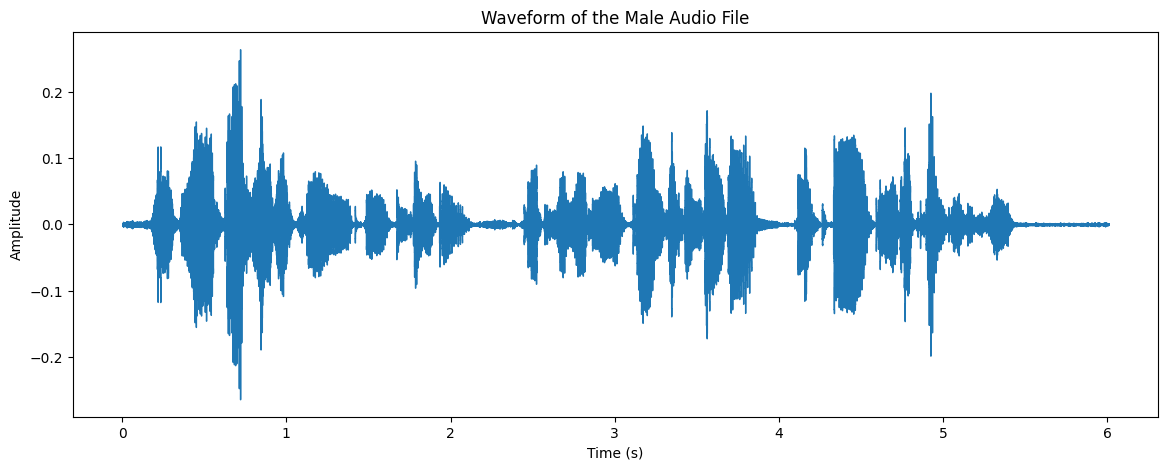
\includegraphics[width=4 in]{Dataset-Male.png}
    \caption{Male Audio Signal as Waveform}
    \label{fig:Dataset-Male}
\end{figure}

\begin{figure}
    \centering
    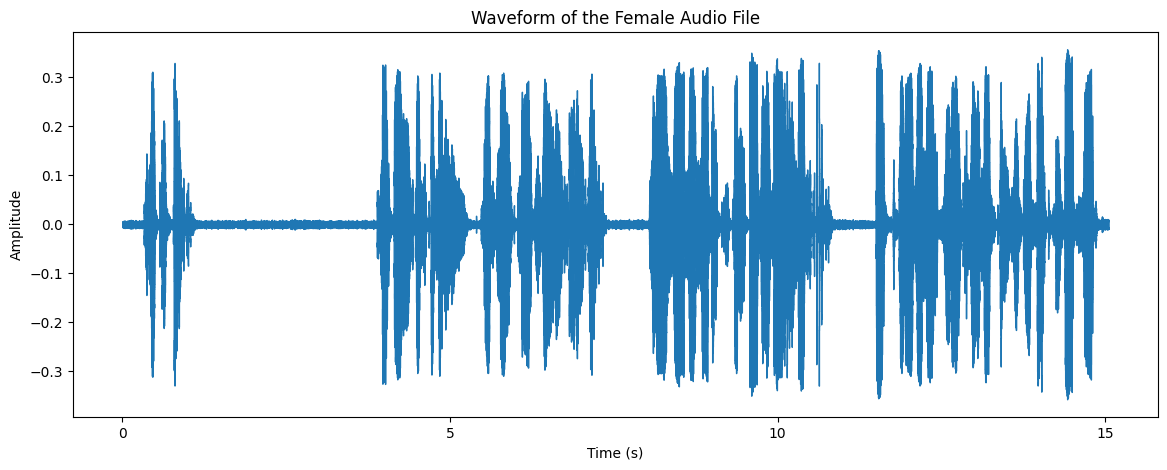
\includegraphics[width=4 in]{Dataset-Female.png}
    \caption{Female Audio Signal as Waveform}
    \label{fig:Dataset-Female}
\end{figure}

This study seeks to provide a comprehensive evaluation of these architectures by comparing their performance on a standardized voice dataset. Through the analysis of metrics such as accuracy, precision, recall, and computational efficiency, this research aims to identify the most effective model for real-world applications. Additionally, the study explores the implications of model complexity, training time, and resource requirements, offering insights into the practical deployment of these technologies.

The findings of this research are expected to contribute to the advancement of voice-based recognition systems by providing a detailed understanding of the strengths and limitations of each architecture. This comparative study will serve as a valuable resource for researchers and practitioners aiming to develop more accurate and efficient voice recognition systems tailored to specific demographic characteristics.

The document is organized into several key sections. Section II provides an extensive review of established models and research on the subject, offering valuable insights that help identify areas for improvement, gaps in current knowledge, and alternative strategies. This section also presents evidence supporting the effectiveness of the proposed solution or highlights possible challenges. Section III describes the implemented model, while Section IV outlines the dataset used for both testing and training. Section V summarizes the report's findings and includes a summary of results along with suggestions for future research directions.

\section{Related work}
In this section, we divide our discussion into two parts: one focusing on research employing similar methods, and the other on research utilizing similar technologies.
\subsection{Research Using Similar Methods}
This subsection reviews previous research utilizing similar acoustic and prosodic methods for speaker age and gender identification. Age estimation from speech has garnered increased interest due to its applications in user profiling, targeted marketing, and personalized call routing, which benefit from real-time capabilities. Long short-term memory (LSTM) recurrent neural networks (RNNs) have outperformed state-of-the-art methods in related speech tasks requiring accurate real-time responses. This paper, authored by Ruben Zazo et al~\cite{zazo2018age}, proposes a novel age estimation system based on LSTM-RNNs that handles short utterances (3 to 10 seconds) and can be deployed in real-time architectures. Tested against a state-of-the-art i-vector approach using NIST speaker recognition evaluation 2008 and 2010 data sets, the proposed system shows up to a 28\% relative improvement in mean absolute error for short-duration utterances.

Abhishek Singhal and Devendra Kumar Sharma~\cite{abdi2010principal} explore gender identification from voice signals across different age groups using various classification algorithms. The paper evaluates recall values for genders within teenage, middle, and old age groups, employing Mel Frequency Cepstral Coefficients (MFCCs) as extracted features. Linear Discriminant Analysis (LDA), Recurrent Neural Network Bidirectional Long Short-Term Memory (RNN-BiLSTM), and Support Vector Machine (SVM) algorithms are utilized for classification. Results indicate that RNN exhibits the highest recall values for both male and female genders across different age groups, outperforming SVM and LDA. Specifically, RNN achieves the highest recall values for males in the teenage group and for females in the old age group, surpassing other algorithms in accuracy as well.

Yong Yu, Xiaosheng Si, Changhua Hu, and Jianxun Zhang~\cite{yu2019review} explore the advancements and applications of long short-term memory (LSTM) in the field of recurrent neural networks (RNNs). While traditional RNNs with sigma or tanh cells struggle with learning relevant information when there are large gaps in the input data, LSTMs address this issue effectively through gate functions that manage long-term dependencies. Since their introduction, LSTMs have achieved significant results and have become central to deep learning research. The paper reviews LSTM cells and their variants, categorizing LSTM networks into LSTM-dominated and integrated LSTM networks, and discusses their diverse applications. Future research directions for LSTM networks are also presented.

Vinayak Sudhakar Kone et al.~\cite{kone2023voice} explore a machine learning-based approach for gender and age detection using voice data. We investigate various feature extraction techniques and evaluate different machine-learning algorithms for classification. We discuss this research area's potential benefits and challenges and highlight open issues for future exploration. Their proposed method utilizes a grid search pipeline with RobustScaler~\cite{qian2022robustscaler}, Principal Component Analysis (PCA)~\cite{abdi2010principal}, and Logistic Regression~\cite{lavalley2008logistic} for age prediction. For gender classification, we employ a sequential model with five hidden layers. This approach achieved an accuracy of 91\% for gender and 59\% for age on the Common Voice dataset.

Ming Li et al. \cite{li2013automatic} presents a novel approach to automatic speaker age and gender identification by combining seven methods at acoustic and prosodic levels to improve baseline performance. The baseline subsystems include Gaussian mixture model (GMM) with mel-frequency cepstral coefficients, support vector machine (SVM) with GMM mean supervectors, and an SVM with 450-dimensional utterance-level features. Four new subsystems are introduced, involving SVMs and sparse representations using various supervectors and prosodic features. These new subsystems effectively classify age and gender groups, and their weighted fusion enhances overall performance. Tested on the 2010 Interspeech Paralinguistic Challenge~\cite{velichko2022complex} a Gender database, the fusion system improves unweighted accuracy by 5.6\% for age and 4.2\% for gender on the development set, and by 3.1\% and 3.8\% respectively on the final test set, compared to the baseline.

\subsection{Research Using Similar Technology}
This subsection explores different technologies used for voice-based age and gender detection. Sera Kim and Seok-Pil Lee present a study focusing on advancing emotion recognition from speech using dimensionality reduction algorithms for visualization to highlight emotion-specific audio features \cite{kim2023bilstm}. The proposed model architecture combines bidirectional long short-term memory (BiLSTM)–Transformer and a 2D convolutional neural network (CNN). The BiLSTM–Transformer captures speech pattern sequences, while the 2D CNN handles Mel-Spectrograms for spatial audio details. Validated using 10-fold cross-validation, the model achieves high unweighted accuracy rates of 95.65\% and 80.19\% on Emo-DB and RAVDESS databases, respectively. These findings suggest that the proposed transformer-based deep learning model, coupled with appropriate feature selection, significantly enhances emotion recognition from speech.

Li-Min Zhang and colleagues explore how gender differences in speech affect emotion recognition~\cite{zhang2023deep} accuracy, proposing a method to improve it by using gender-specific features. The study begins with classifying speech by gender using a Multi-Layer Perceptron (MLP). It then analyzes the impact of various acoustic features on emotion recognition for male and female speech, establishing optimal feature sets for each gender. These sets are used to train and test Convolutional Neural Networks (CNN) and Bidirectional Long Short-Term Memory networks (BiLSTM). The results demonstrate that the proposed gender-specific emotion recognition models outperform gender-mixed models in terms of average recognition accuracy.

Sidra Abid Syed discusses the role of computerized acoustic examination in early diagnosis and monitoring of pathological speech~\cite{syed2021comparative}. The study aims to detect diseases from voice using various acoustic metrics, which are influenced by speech noise detection algorithms. The methodology involves feature extraction from the SVD dataset, followed by input into a 27-layer neural network comprising convolutional and recurrent layers. The dataset is divided for training and testing, and 10-fold cross-validation is employed to assess performance. The reported accuracies are 87.11\% for CNN and 86.52\% for RNN. The program, written in Python using TensorFlow, was executed on a Linux workstation with an NVidia Titan X GPU.
\section{Proposed Method}

\begin{figure}
    \centering
    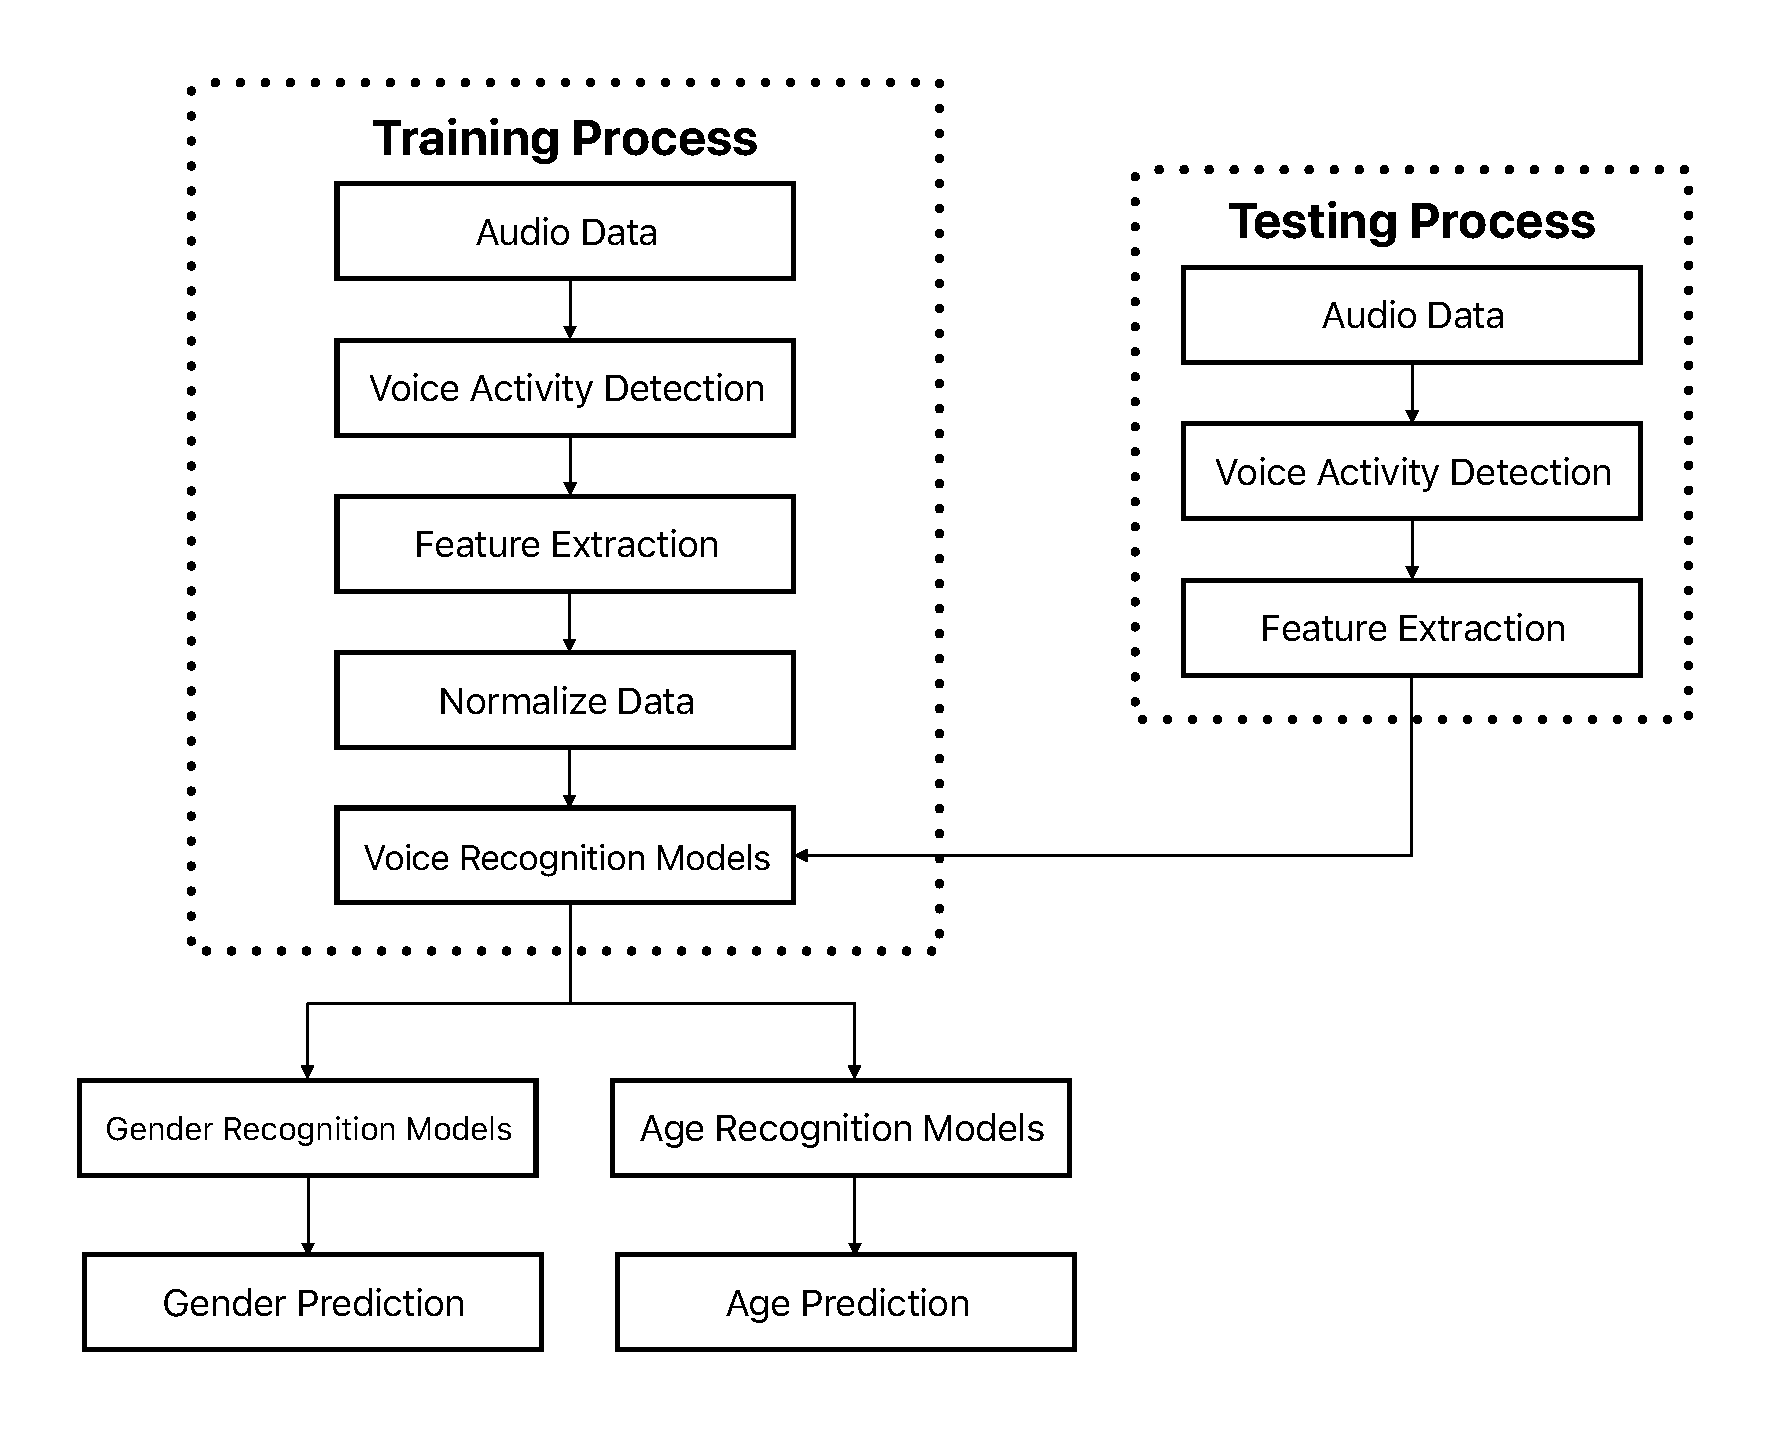
\includegraphics[width=3.5 in]{Research Architecture.pdf}
    \caption{Architecture of Voice based Age and Gender Recognize System}
    \label{fig:Research Architecture}
\end{figure}

\subsection{Sound Extraction}
\subsubsection{Mel-frequency cepstral coefficients (MFCC)}
\subsubsection{Picth and Magnitude}
\subsubsection{Filter - Bank Energies}

\subsection{Architecture}
\subsubsection{Long Short Term Memory Architecture}
\begin{figure}
    \centering
    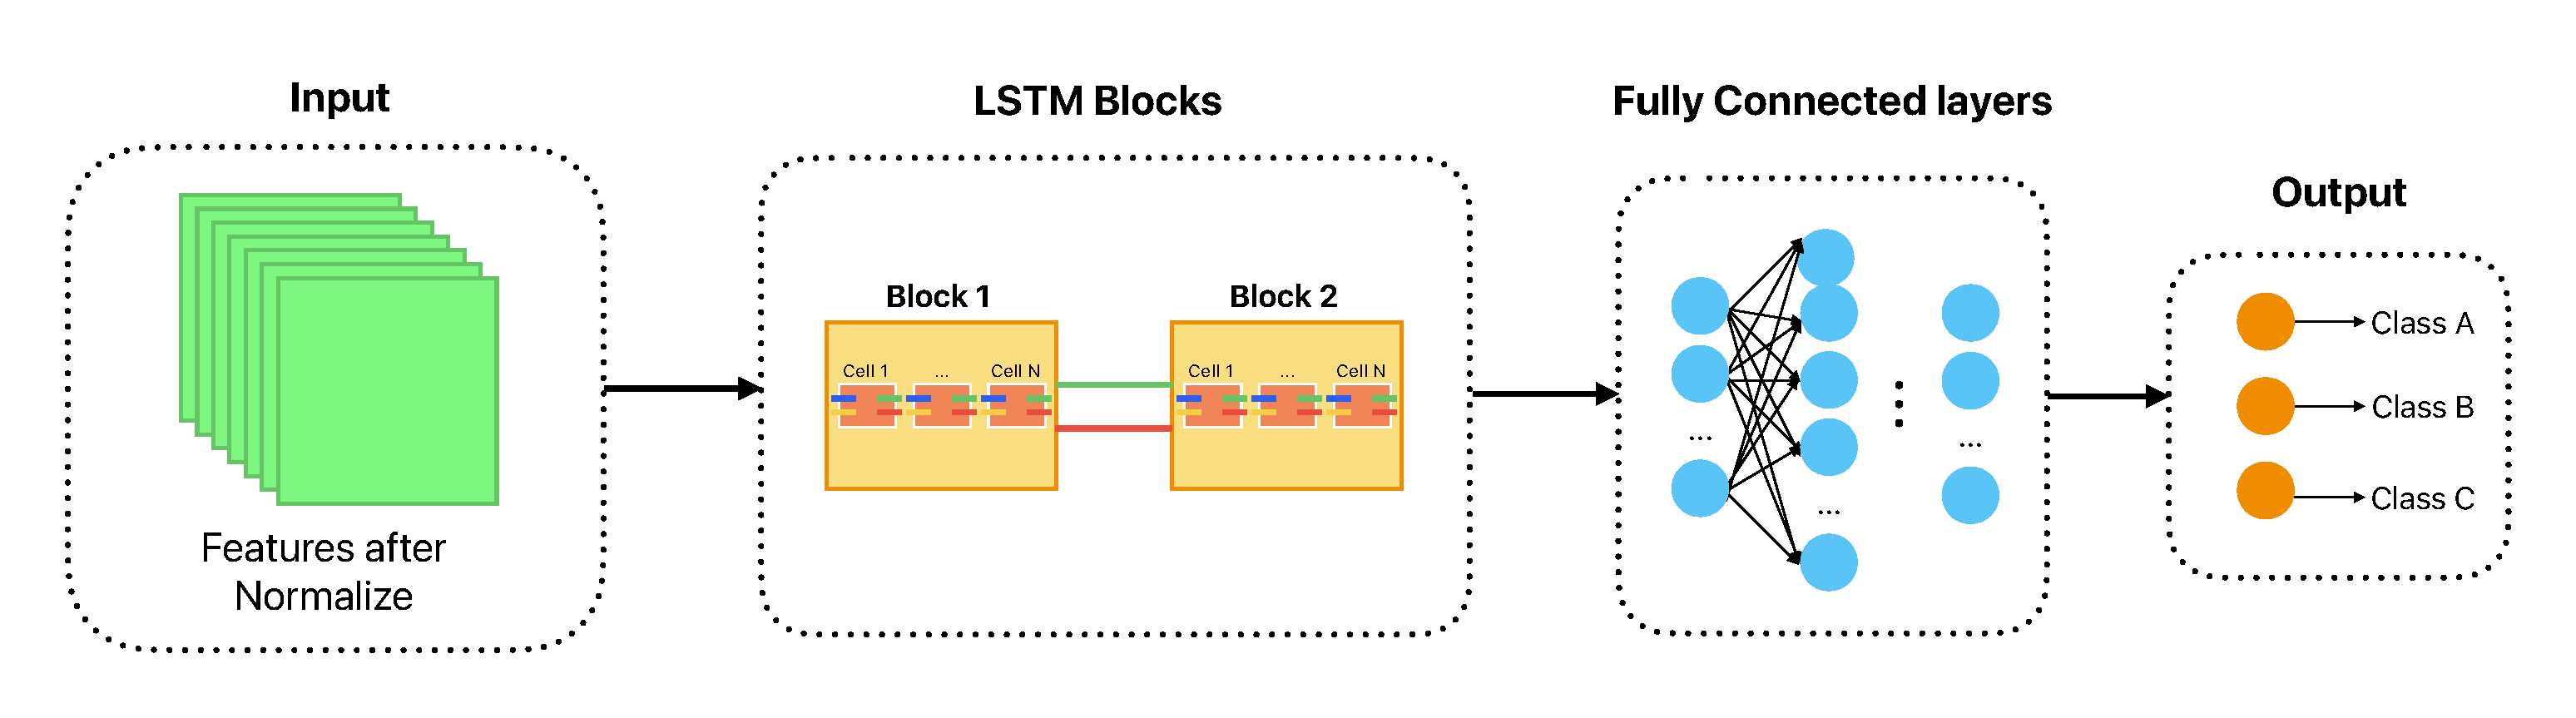
\includegraphics[width=7 in]{LSTM architecture.pdf}
    \caption{LSTM Architecture}
    \label{fig:LSTM architecture}
\end{figure}
\begin{figure}
    \centering
    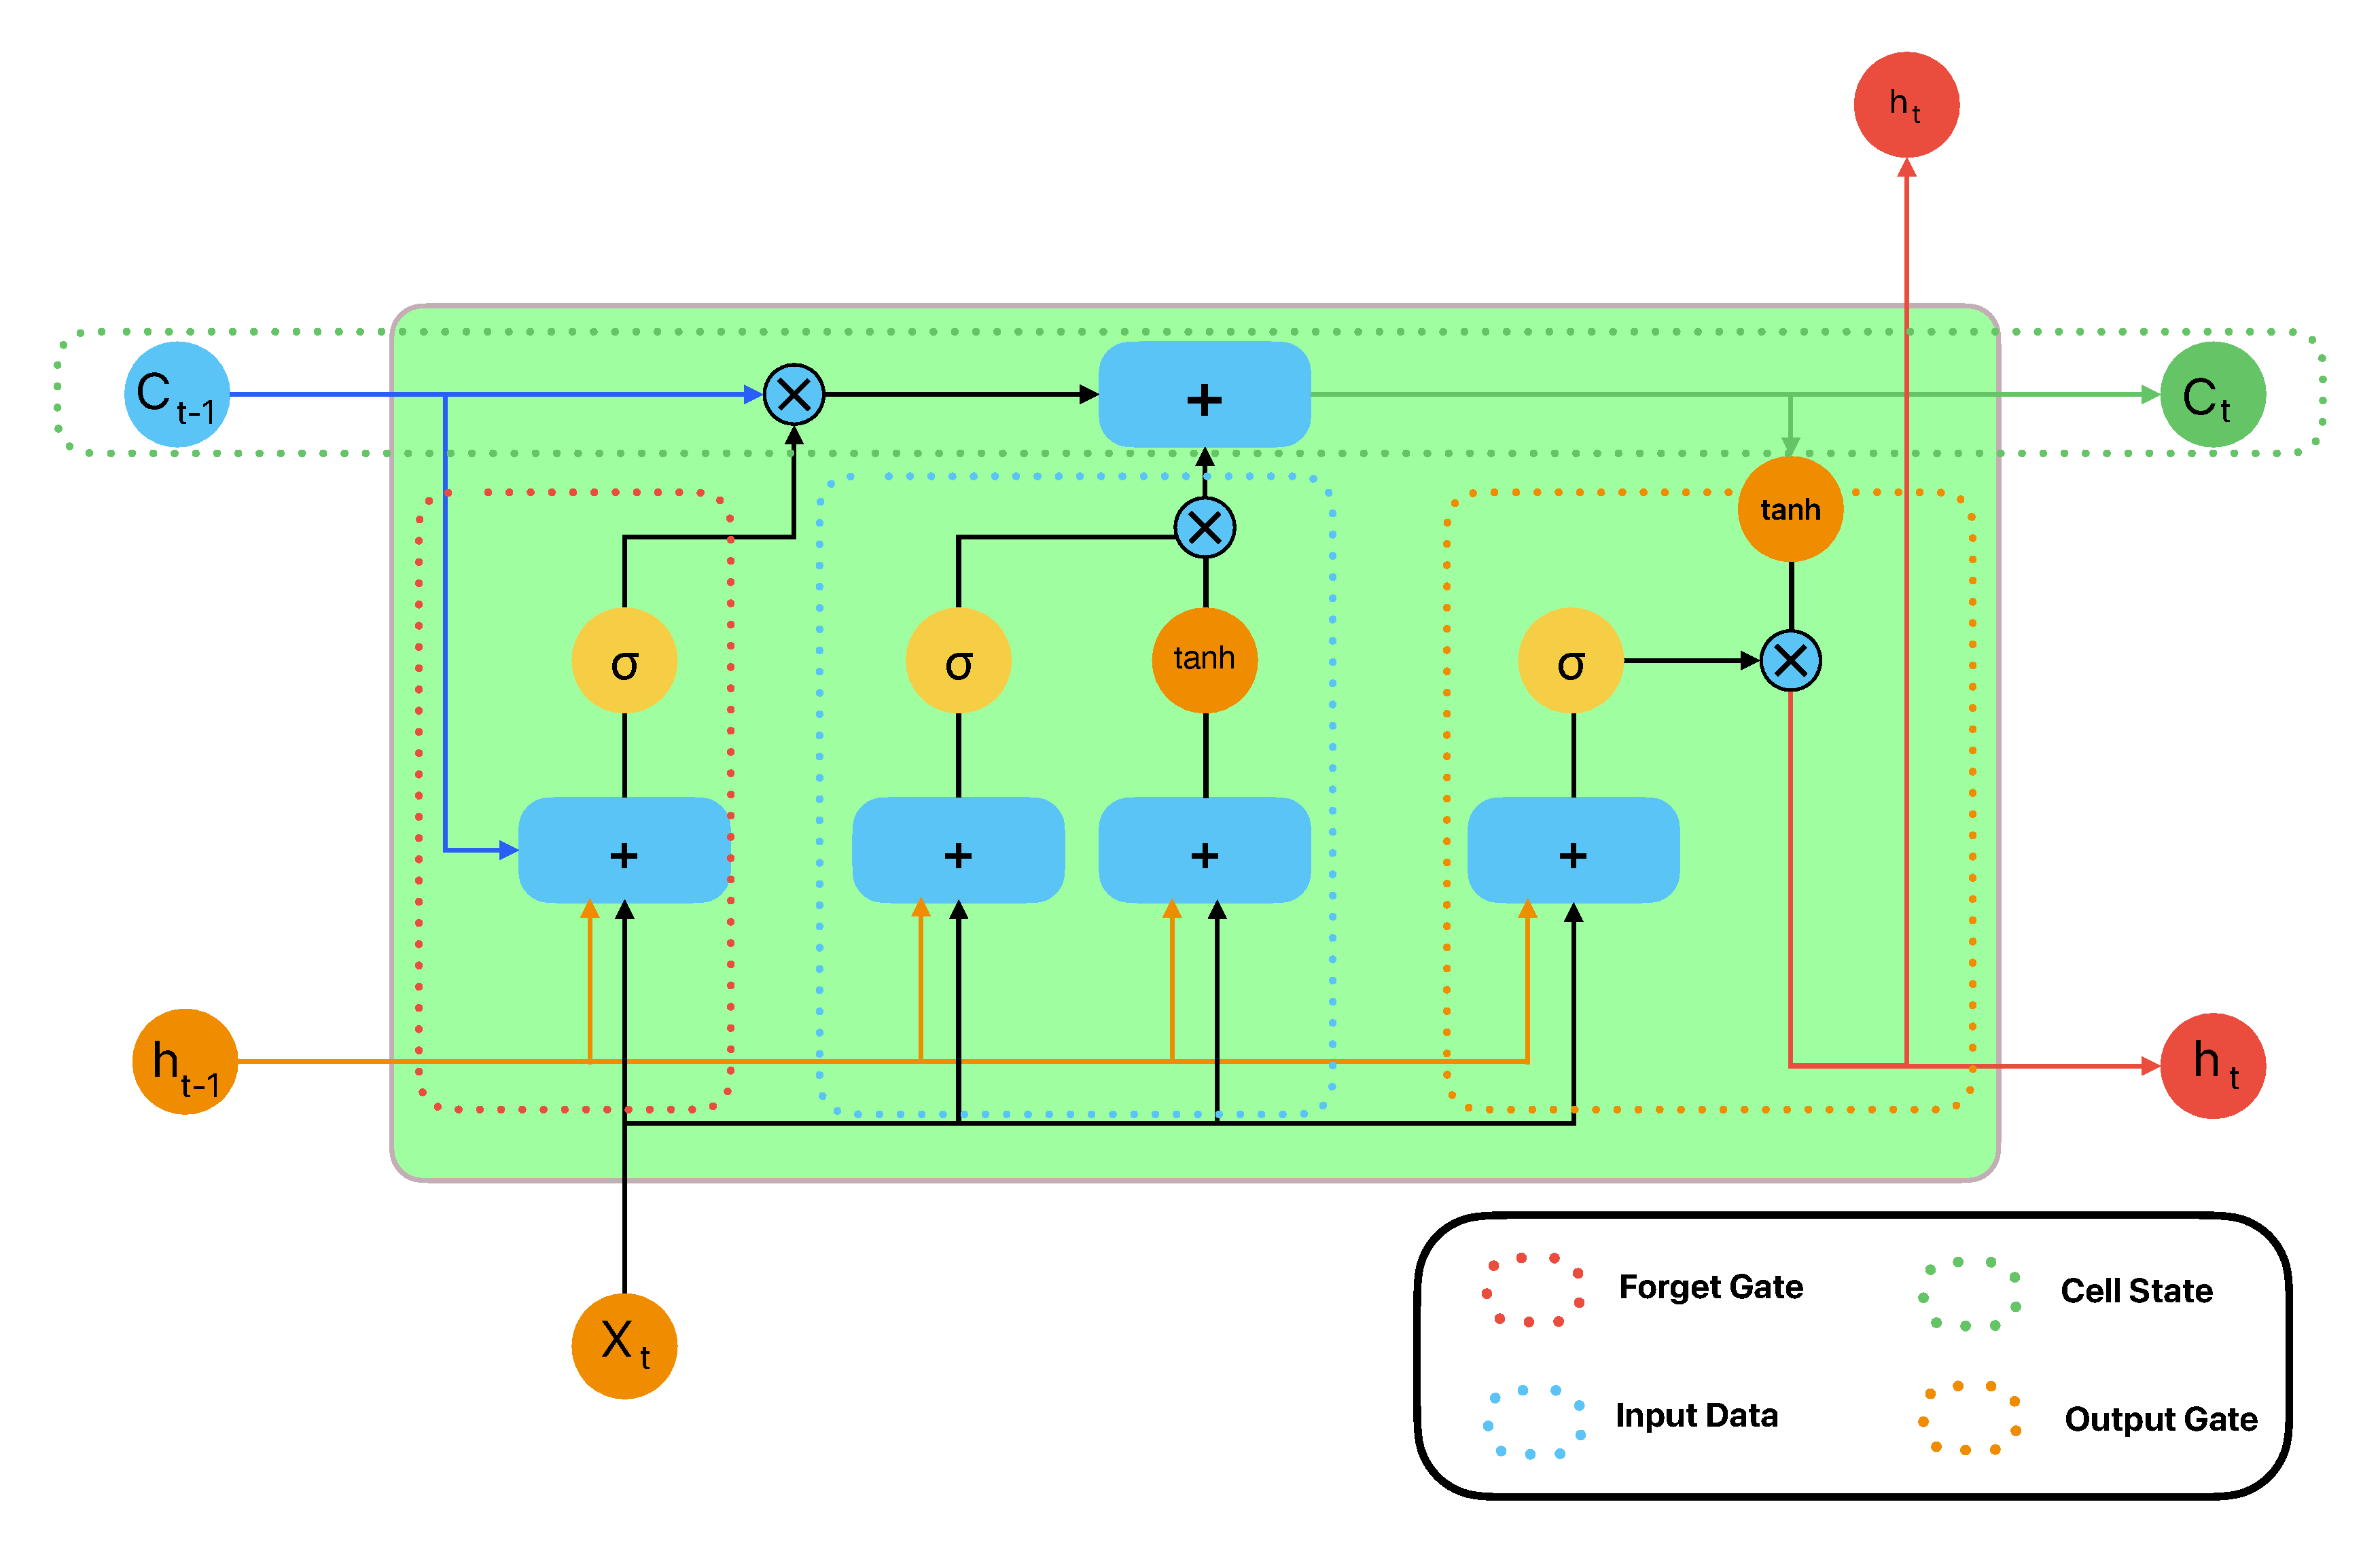
\includegraphics[width=4 in]{LSTM cell architecture.pdf}
    \caption{LSTM Cell architecture}
    \label{fig:LSTM cell architecture}
\end{figure}
\subsubsection{RezoNet Architecture}
\begin{figure}
    \centering
    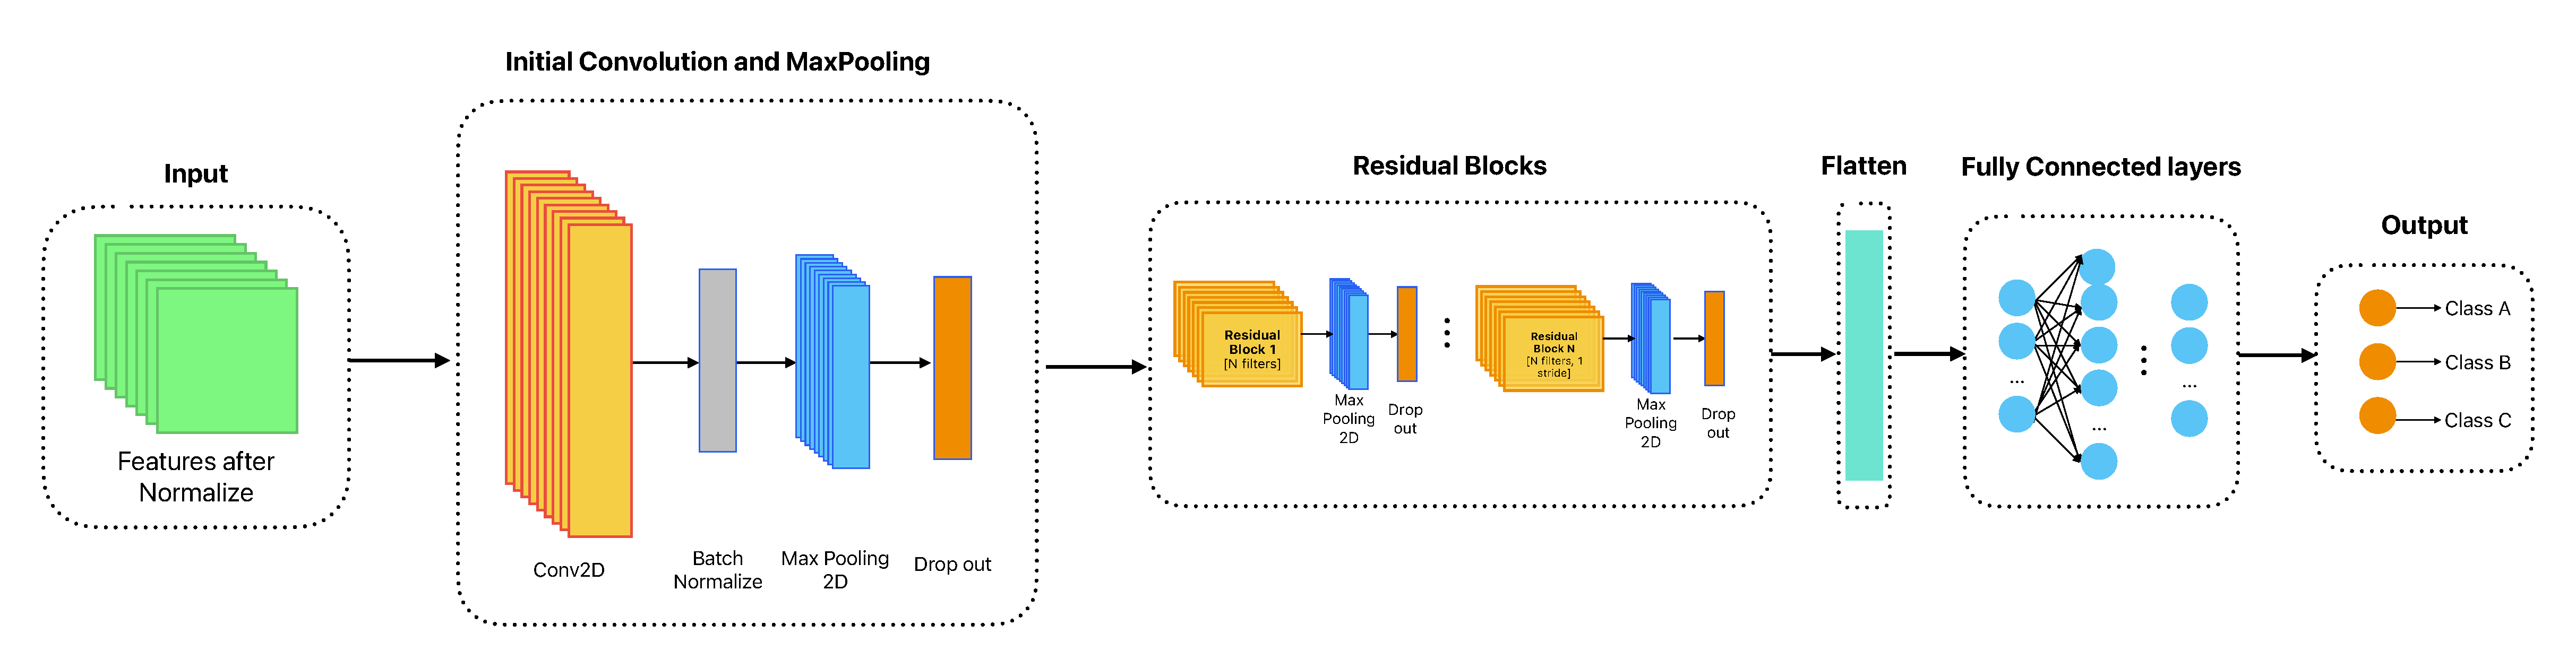
\includegraphics[width=7 in]{RezoNet Architecture.pdf}
    \caption{RezoNet Architecture}
    \label{fig:RezoNet Architecture}
\end{figure}
\begin{figure}
    \centering
    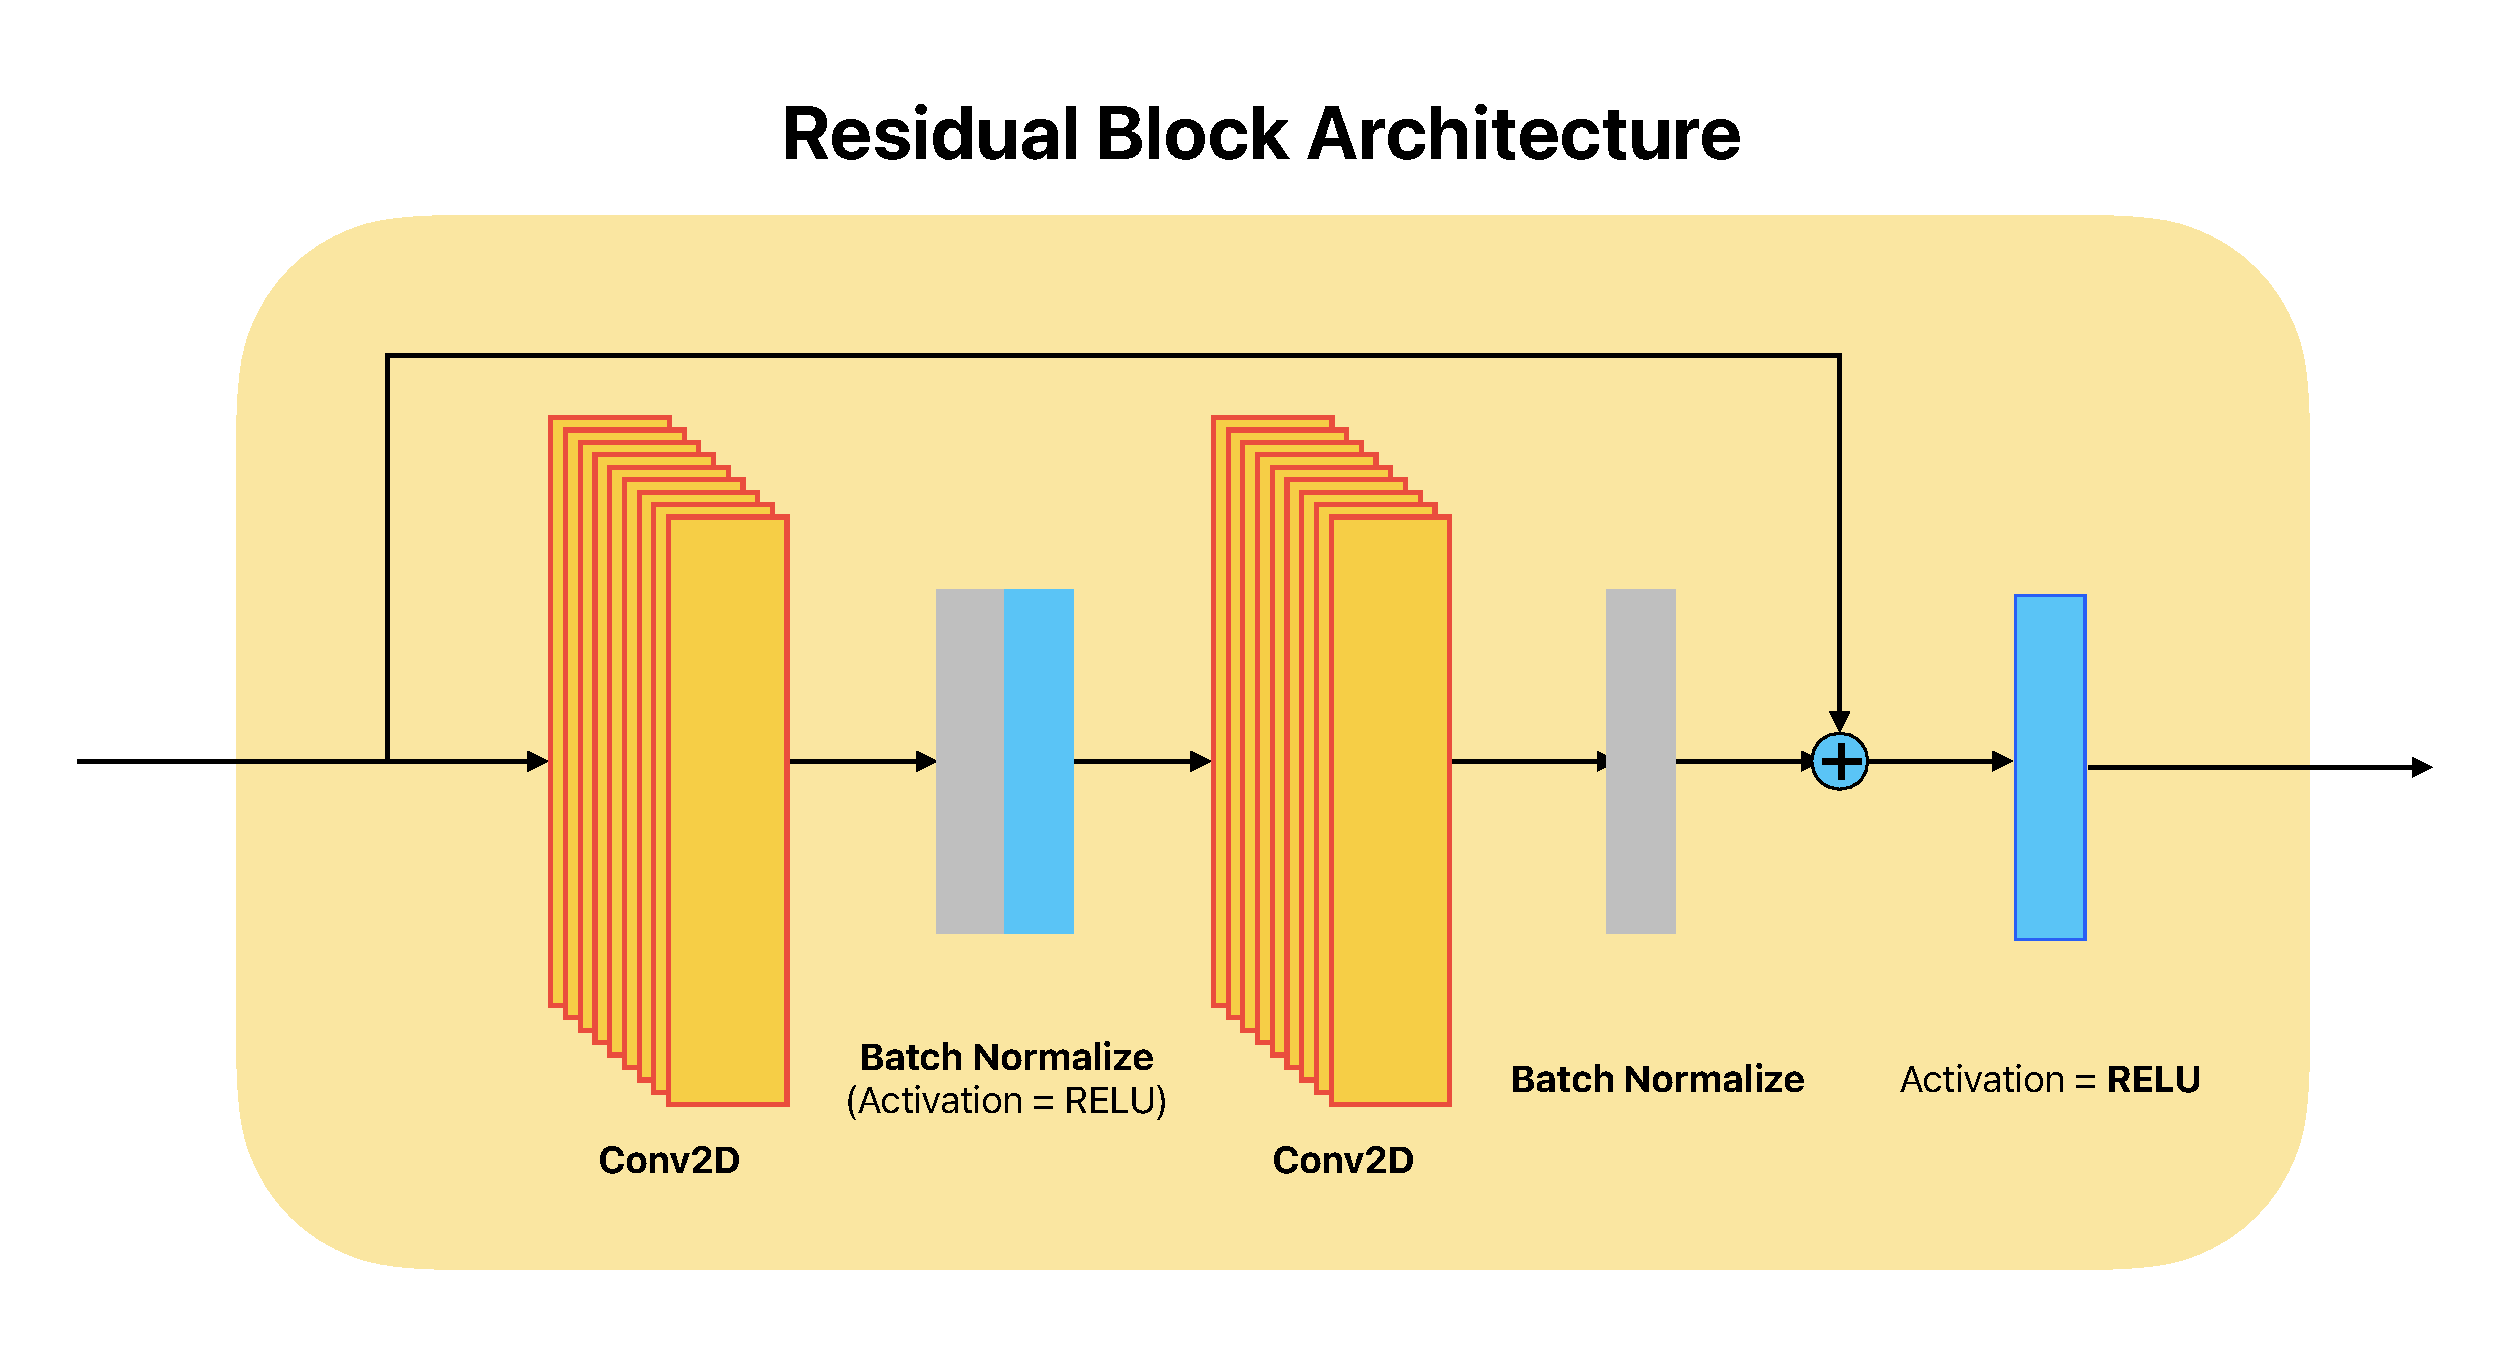
\includegraphics[width=4 in]{Residual Block Architecture.pdf}
    \caption{Residual Block Architecture}
    \label{Residual Block Architecture}
\end{figure}
\subsubsection{CNN -BiLSTM Architecture}
\begin{figure}
    \centering
    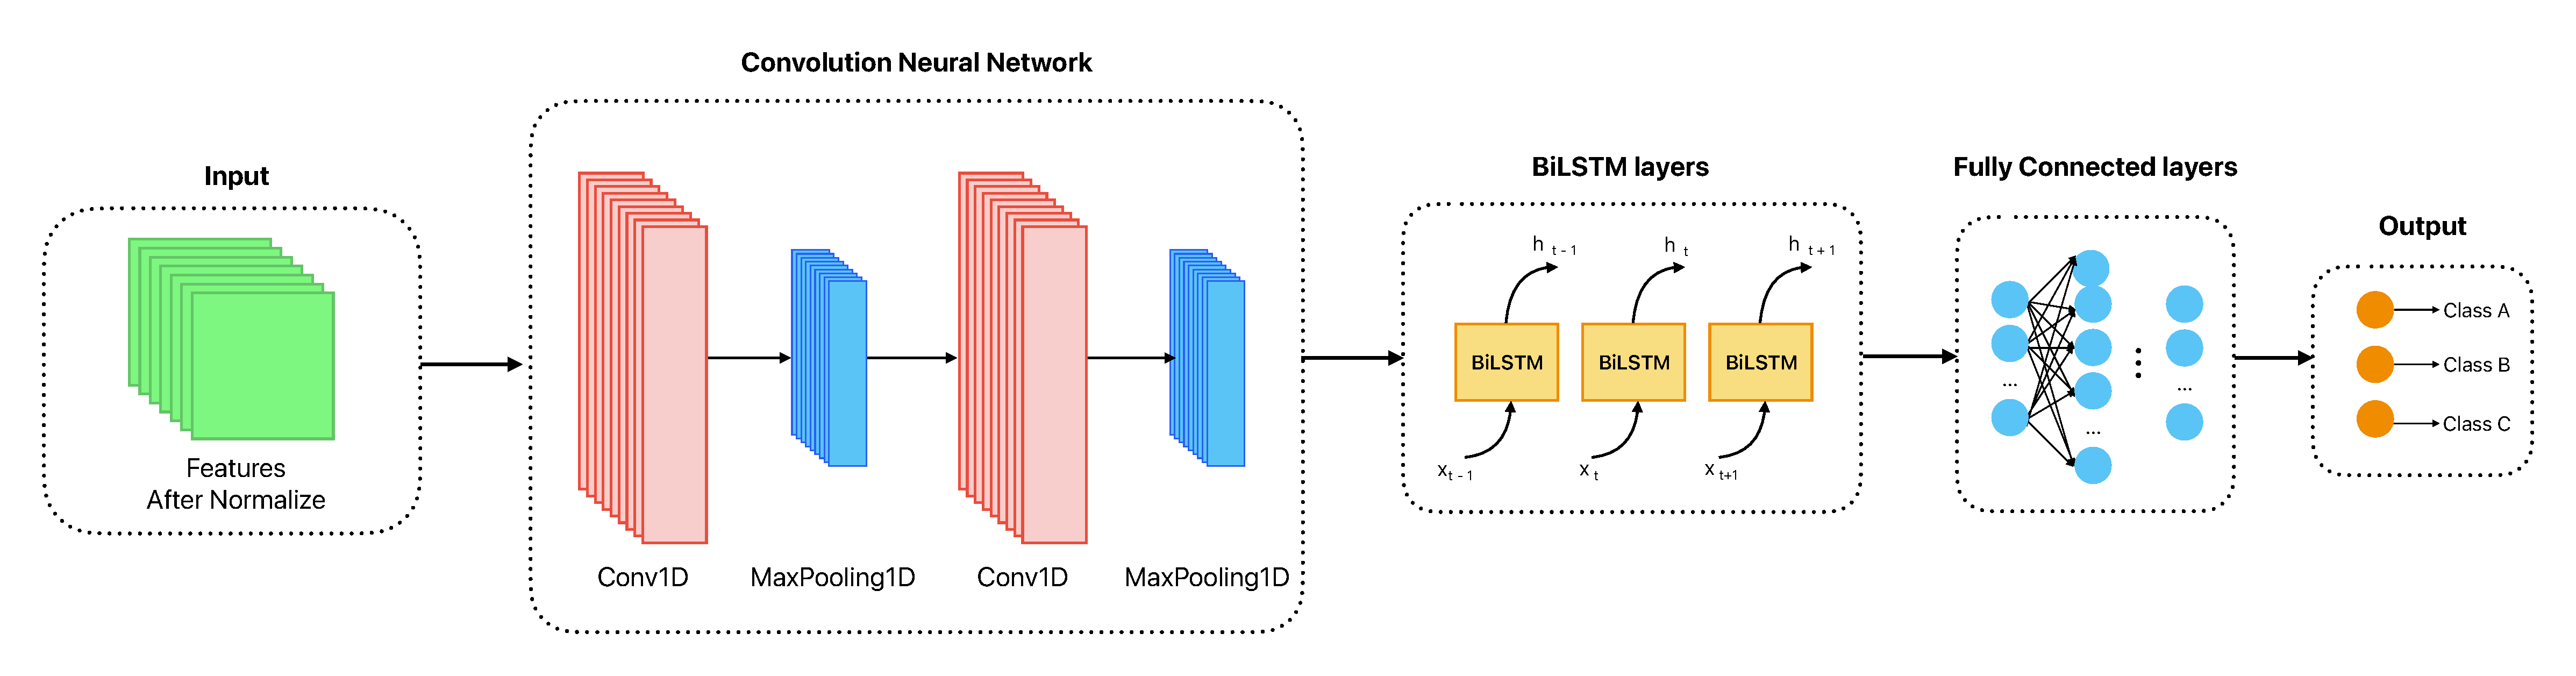
\includegraphics[width=7 in]{CNN-BiLSTM architecture.pdf}
    \caption{CNN - BiLSTM Hybrid Architecture}
    \label{fig:CNN - BiLSTM Hybrid Architecture}
\end{figure}

\subsection{Performance Matrix}

\section{Experimental Result and Discussion}
\subsection{Experiment settings}

The training process is conducted on a personal computer equipped with an Intel® Core™ i7-12650H processor, and an NVIDIA GeForce RTX 3060 GPU with 8GB of RAM.
\subsection{Dataset}
\subsubsection{Dataset for Gender Recognition Model}

After The Mozilla Voice Dataset~\cite{mozilla_voice} cleansing procedures, we homogenized the dataset to solely include male and female classifications. Subsequently, we partitioned this refined dataset into subsets suitable for Gender Recognition Modeling, totaling %8,000
items. This allocation comprised %5,400
entries designated for training purposes, %600
for validation, and %2,000 
for testing. Notably, each subset maintained a balanced representation of genders, with male and female categories accounting for 50\% and 50\% of the data, respectively. It is represented through in Table~\ref{tab:Distribution of samples in the Gender dataset}.

\begin{table}[htbp]
    \centering
    \begin{tabular}{|c|ccc|}
    \hline
    \textbf{Category} & \textbf{Train Dataset} & \textbf{Valid Dataset} & \textbf{Test Dataset}\\
    \hline
    Male & 4000 & 1000 & 500 \\
    Female & 4000 & 1000 & 500 \\
    \hline
    \textbf{Total} & 8000 & 2000 & 1000 \\
    \hline
    \end{tabular}
    \caption{Distribution of samples in the Gender dataset}
    \label{tab:Distribution of samples in the Gender dataset}
\end{table}

\subsubsection{Dataset for Age Recognition Model}
 Following the Mozilla Voice Dataset~\cite{mozilla_voice} refinement processes, we standardized the dataset to encompass five age categories. Subsequently, we partitioned this refined dataset into subsets tailored for age-based modeling, totaling %8,000 
 items. This allocation included %13,279 
 entries designated for training purposes, %1,476 
 entries for validation, and %790 
 entries for testing. It is noteworthy that each subset retained a balanced representation across five age classifications: teens, twenties, thirties, forties, and fifties to sixties. It is represented through Table~\ref{tab:Distribution of samples in the Age dataset}.

\begin{table}[htbp]
    \centering
    \begin{tabular}{|c|ccc|}
    \hline
    \textbf{Category} & \textbf{Train Dataset} & \textbf{Valid Dataset} & \textbf{Test Dataset}\\
    \hline
    Teens & 2361 & 590 & 160 \\
    Twenties & 2361 & 591 & 160 \\
    Thirties & 2361 & 590 & 160 \\
    Forties & 2361 & 590 & 160 \\
    Fifties - Sixties & 2360 & 590 & 160 \\
    \hline
    \textbf{Total} & 11804 & 2951 & 800\\
    \hline
    \end{tabular}
    \caption{Distribution of samples in the Age dataset}
    \label{tab:Distribution of samples in the Age dataset}
\end{table}
\subsection{Feature Extraction}             %Visualize feature extraction

\begin{table}[htbp]
    \centering
    \begin{tabular}{|c|c|}
        \hline
        \textbf{Sound processing} & \textbf{Feature} \\
        \hline
        Delta MFCC & 13 \\
        Delta delta MFCC & 13\\
        Picth & 1 \\
        Magnitude & 1 \\ 
        Filter - Bank Energies & 26\\
        \hline
        \textbf{Total} & \textbf{54} \\
        \hline 
    \end{tabular}
    \caption{Feature Extraction}
    \label{tab:Feature Extraction}
\end{table}

\subsection{Models' Architecture}
\subsubsection{Long - Short Term Memory (LSTMs) architecture}

\begin{table}[htbp]
    \centering
    \begin{tabular}{|c|cccc|}
        \hline
        \textbf{Class} & \textbf{Precision} & \textbf{Recall} & \textbf{F1-score} & \textbf{Support} \\
        \hline
        Male & 0.96178 & 0.90600 & 0.93306 & 500 \\
        Female & 0.91115 & 0.96400 & 0.93683 & 500 \\
        \hline
        \textbf{Accuracy} & \multicolumn{2}{c}{} & 0.93500 & 1000 \\
        \textbf{Macro Average} & 0.93647 & 0.93500 & 0.93495 & 1000 \\
        \textbf{Weighted Average} & 0.93647 & 0.93500 & 0.93495 & 1000 \\
        \hline
    \end{tabular}
    \caption{Experience of Gender Recognize Model with LSTMs Architecture}
    \label{tab:Experience of Gender Recognize Model with LSTM Architecture}
\end{table}

\begin{table}[htbp]
    \centering
    \begin{tabular}{|c|cccc|}
        \hline
        \textbf{Class} & \textbf{Precision} & \textbf{Recall} & \textbf{F1-score} & \textbf{Support} \\
        \hline
        Teens & 0.67227 & 0.64375 & 0.66883 & 160 \\
        Twenties & 0.49763 & 0.65625 & 0.56604 & 160 \\
        Thirties & 0.65746 & 0.74375 & 0.69795 & 160 \\
        Forties & 0.75887 & 0.66875 & 0.71096 & 160 \\
        Fifties - Sixties& 0.69595 & 0.64375 & 0.66883 & 160 \\
        \hline
        \textbf{Accuracy} &  && 0.64250 & 800 \\
        \textbf{Macro Average} & 0.65643 & 0.64250 & 0.64345 & 800 \\
        \textbf{Weighted Average} & 0.65643 & 0.64250 & 0.64345  & 800 \\
        \hline
    \end{tabular}
    \caption{Experience of Age Recognize Model with LSTMs Architecture}
    \label{tab:Experience of Age Recognize Model with LSTMs Architecture}
\end{table}
\subsubsection{RezoNet Architecture}

\begin{table}[htbp]
    \centering
    \begin{tabular}{|c|cccc|}
        \hline
        \textbf{Class} & \textbf{Precision} & \textbf{Recall} & \textbf{F1-score} & \textbf{Support} \\
        \hline
        Male & 0.96884 & 0.68400 & 0.80188 & 500 \\
        Female & 0.75580 & 0.97800 & 0.85266 & 500 \\
        \hline
        \textbf{Accuracy} & \multicolumn{2}{c}{} & 0.83100 & 1000 \\
        \textbf{Macro Average} & 0.86232 & 0.83100 & 0.82727 & 1000 \\
        \textbf{Weighted Average} &0.86232 & 0.83100 & 0.82727  & 1000 \\
        \hline
    \end{tabular}
    \caption{Experience of Gender Recognize Model with RezoNet Architecture}
    \label{tab:Experience of Gender Recognize Model with RezoNet Architecture}
\end{table}

\begin{table}[htbp]
    \centering
    \begin{tabular}{|c|cccc|}
        \hline
        \textbf{Class} & \textbf{Precision} & \textbf{Recall} & \textbf{F1-score} & \textbf{Support} \\
        \hline
        Teens & 0.52475 & 0.33125 & 0.40613 & 160 \\
        Twenties & 0.32919 & 0.33125 & 0.33022 & 160 \\
        Thirties & 0.41071 & 0.71875 & 0.52273 & 160 \\
        Forties & 0.48148 & 0.40625 & 0.44068 & 160 \\
        Fifties - Sixties& 0.59350 & 0.45625 & 0.51590 & 160 \\
        \hline
        \textbf{Accuracy} &  &  & 0.44875 & 800 \\
        \textbf{Macro Average} & 0.46793 & 0.44875 & 0.44313 & 800 \\
        \textbf{Weighted Average} & 0.46793 & 0.44875 & 0.44313  & 800 \\
        \hline
    \end{tabular}
    \caption{Experience of Age Recognize Model with RezoNet Architecture}
    \label{tab:Experience of Age Recognize Model with RezoNet Architecture}
\end{table}

\subsubsection{CNN-BiLSTM Hybrid Architecture}

\begin{table}[htbp]
    \centering
    \begin{tabular}{|c|cccc|}
        \hline
        \textbf{Class} & \textbf{Precision} & \textbf{Recall} & \textbf{F1-score} & \textbf{Support} \\
        \hline
        Male & 0.93535 & 0.92600 & 0.93065 & 500 \\
        Female & 0.92673 & 0.93600 & 0.93134 & 500 \\
        \hline
        \textbf{Accuracy} & \multicolumn{2}{c}{} & 0.93100 & 1000 \\
        \textbf{Macro Average} & 0.93104 & 0.93100 & 0.93100 & 1000 \\
        \textbf{Weighted Average} & 0.93104 & 0.93100 & 0.93100 & 1000 \\
        \hline
    \end{tabular}
    \caption{Experience of Gender Recognize Model with CNN - BiLSTM Hybrid Architecture}
    \label{tab:Experience of Gender Recognize Model with CNN - BiLSTM Hybrid Architecture}
\end{table}

\begin{table}[htbp]
    \centering
    \begin{tabular}{|c|cccc|}
        \hline
        \textbf{Class} & \textbf{Precision} & \textbf{Recall} & \textbf{F1-score} & \textbf{Support} \\
        \hline
        Teens & 0.63871 & 0.61875 & 0.62857 & 160 \\
        Twenties & 0.59281 & 0.61875 & 0.60550 & 160 \\
        Thirties &  0.79054 & 0.73125 & 0.75974 & 160 \\
        Forties &   0.70213 & 0.82500 & 0.75862 & 160 \\
        Fifties - Sixties & 0.70213 & 0.82500 & 0.75862 & 160 \\
        \hline
        \textbf{Accuracy} &  &  & 0.69750 & 800 \\
        \textbf{Macro Average} & 0.70118 & 0.69750 & 0.69751 & 800 \\
        \textbf{Weighted Average} & 0.70118 & 0.69750 & 0.69751 & 800 \\
        \hline
    \end{tabular}
    \caption{Experience of Age Recognize Model with CNN - BiLSTM Hybrid Architecture}
    \label{tab:Experience of Age Recognize Model with CNN - BiLSTM Hybrid Architecture}
\end{table}



\subsection{Comparison Architecture}
\begin{figure}
    \centering
    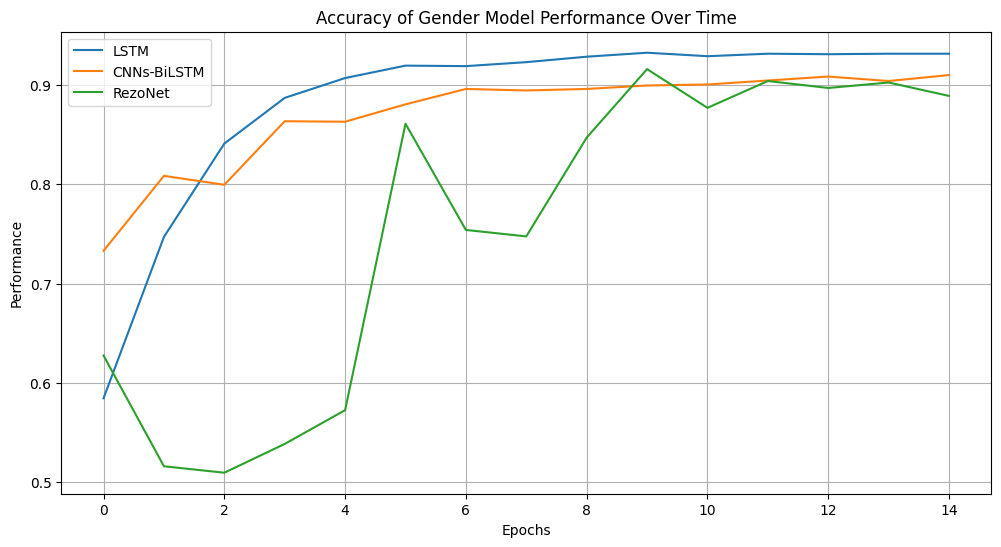
\includegraphics[width=4 in]{Gender_valid.png}
    \caption{Accuracy of Gender Model Performance Over Time}
    \label{fig:Gender_valid}
\end{figure}

\begin{figure}
    \centering
    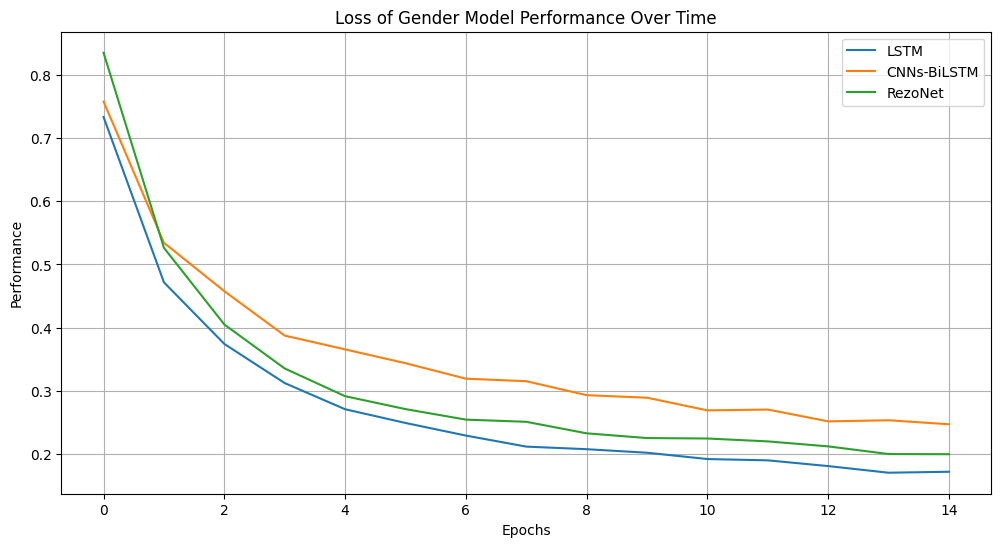
\includegraphics[width=4 in]{Loss_Gender_valid.png}
    \caption{Loss of Gender Model Performance Over Time}
    \label{fig:Loss_Gender_valid}
\end{figure}

\begin{figure}
    \centering
    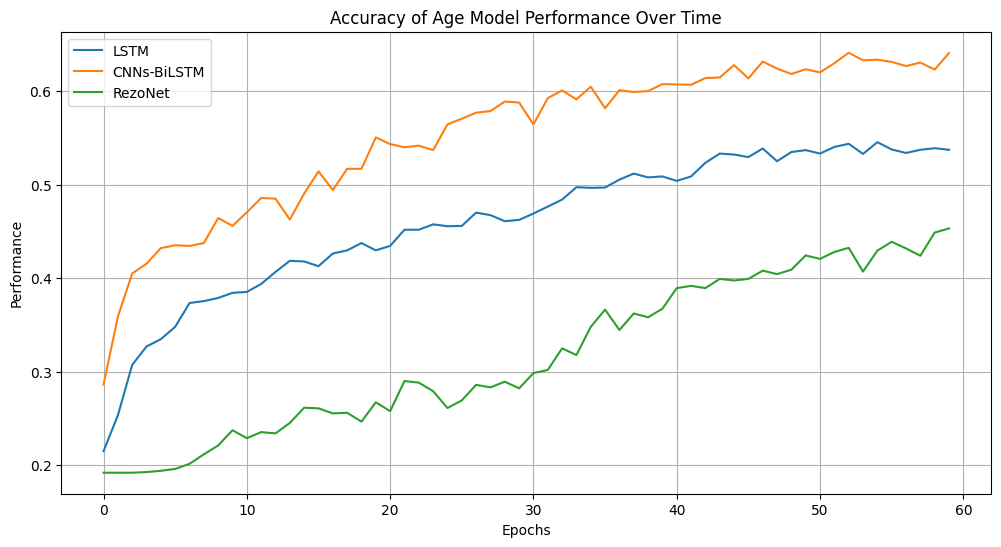
\includegraphics[width=4 in]{Accuracy_Age_valid.png}
    \caption{Accuracy of Age Model Performance Over Time}
    \label{fig:Age_valid}
\end{figure}

\begin{figure}
    \centering
    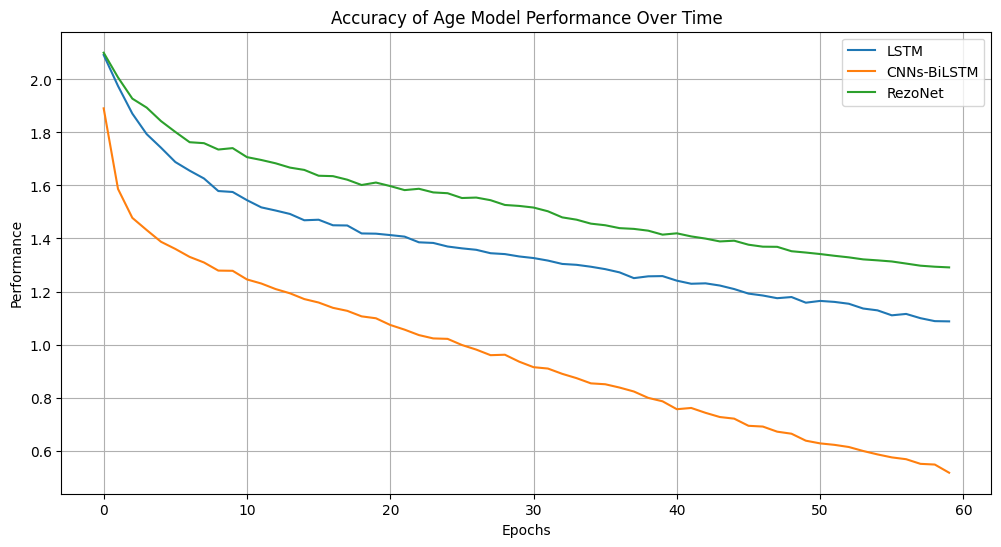
\includegraphics[width=4 in]{Loss_Age_valid.png}
    \caption{Loss of Age Model Performance Over Time}
    \label{fig:Loss_Age_valid}
\end{figure}
\section{Conclusion and Future Enhancements}
\section{Acknowledgment}

\bibliographystyle{IEEEtran}  % IEEE
\bibliography{Mybib}          % IEEE

\end{document}


